%!TEX TS-program = pdflatex
\documentclass[twoside]{article}
\usepackage{waspaa01,amssymb,amsmath,epsfig}
\usepackage{graphicx,mcode}
\usepackage{listings}
\usepackage{verbatim}
\usepackage{url}

%% Now actually use the newly defined style.

\lstset{ %
%language=C,                % choose the language of the code
%basicstyle=\footnotesize,       % the size of the fonts that are used for the code
%numbers=left,                   % where to put the line-numbers
numberstyle=\footnotesize,      % the size of the fonts that are used for the line-numbers
stepnumber=1,                   % the step between two line-numbers. If it's 1 each line will be numbered
numbersep=0pt,                  % how far the line-numbers are from the code
backgroundcolor=\color{white},  % choose the background color. You must add \usepackage{color}
showspaces=false,               % show spaces adding particular underscores
showstringspaces=false,         % underline spaces within strings
showtabs=false,                 % show tabs within strings adding particular underscores
tabsize=2,                      % sets default tabsize to 2 spaces
captionpos=b,                   % sets the caption-position to bottom
breaklines=true,                % sets automatic line breaking
breakatwhitespace=false,        % sets if automatic breaks should only happen at whitespace
escapeinside={\%*}{*)}          % if you want to add a comment within your code
}
\setcounter{page}{1}
%\ninept  % 9-pt size optional (10-pt default)

\title{Veritune: Digital Phase Vocoder}
\name{Chris Li, Grayson Smith, Carey Zhang}
\address{github.com/unregistered/speakurity}

%
\begin{document}
\maketitle
%
\begin{abstract}
	For our EE201 final Verilog project, we attempt to implement a digital phase vocoder on the FPGA. 
	We wrote a 256-point Radix-2 Decimation-in-Time Fast Fourier Transform module, which works in hardware.  
	The phase vocoder allows us to do	the actual pitch shifting. Due to the limited resources on the board,
	we had to implement the phase vocoder in software using \textsc{Matlab}. The software version utilizes a 
	1024 point transform.
\end{abstract}

%
%
% Introduction
%
%
\section{Introduction}
  The phase vocoder has many uses in the music industry, both as a correction tool and as an audio effect.
  When combined with a pitch detection algorithm, it can shift the input signal to the nearest whole pitch, an effect known as auto-tuning.
  If the shift can be performed in under 50 milliseconds, the delay won't be perceptible and can be used for live performances \cite{bib:guitarpitchshifter}.
  

  
%
%
% FFT
%
%
\section{Radix-2 DIT FFT}
  The first component we had to create was the Fast Fourier Transform. The FFT takes a discrete signal in the time domain and 
  transforms it into the frequency domain. For our device we need a 1024 point FFT.
  \subsection{Relevant Theory}
  The Discrete Fourier Transform is shown below.
  \begin{equation}
  	X_k = \sum_{n=0}^{N-1} x_n e^{-\frac{2 \pi j}{N} k n} \quad \quad k = 0, \dots, N-1
  	\label{eqn:dft}
  \end{equation}
  
  However, the number of operations required scales as $N^2$ and the DFT becomes very expensive at 1024 points.
  The Cooley Tukey Algorithm is an Fast Fourier Transform, which reduces the number of operations \cite{bib:ctdft}.
  \begin{equation}
  	 X_k  =	 \sum \limits_{m=0}^{N/2-1} x_{2m}     e^{-\frac{2\pi j}{N} (2m)k}\\   +  \sum \limits_{m=0}^{N/2-1} x_{2m+1} e^{-\frac{2\pi j}{N} (2m+1)k}
  	\label{eqn:ctdft}
  \end{equation} 
  
  \subsection{Hardware Implementation}
  Because the number of points is a power of two, we can use Radix-2 Decimation in Time.
  The Cooley Tukey Algorithm can be applied recursively until the size of the FFT is 2.  
  The dataflow for our algorithm is shown in figure \ref{fig:butterfly}.  Each column
  is called a pass, each set of interlocked rows in the pass is a block, and each pair of lines is called a 
  butterfly (after the appearance of crossing lines).
  \begin{figure}[h]
  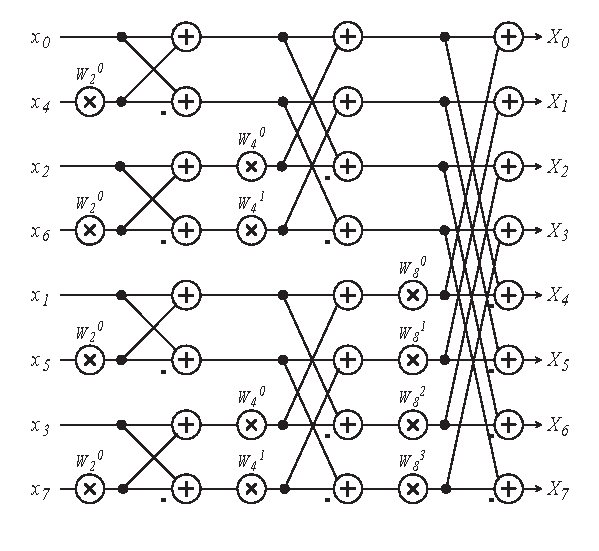
\includegraphics[width=75mm]{images/butterfly.pdf}
  \caption{Dataflow of radix-2 DIT FFT \cite{bib:butterfly}. $W_k^n$ represents the Twiddle factor $e^{-\frac{2\pi j}{N}kn}$.}  
  \label{fig:butterfly}
  \end{figure}
  
  We have chosen this algorithm for the substantial savings in operations. The number of complex multiplies and adds in
  the Radix-2 DIT FFT scales as $Nlog(N)$. In theory, a 1024 point DFT requires 1048576 multiplies while the FFT uses 
  only 5120 \cite{bib:fftdit}.
  
  The FFT requires us to compute a complex exponential, which can be expressed as a sine and cosine.  One option would be to 
  implement CORDIC for calculating trigonometric functions.  However, the exponential is a function of only current indexes.  
  Therefore, we implemented it as a look up table with 512 elements (the function is symmetric).  The elements in the LUT
  are called Twiddle Factors. 
  
  Another feature of this implementation is the bit re-ordering, as shown in the figure. Because the algorithm computes the
  FFT in-place, we must re-order the input data.  On software systems this is less desirable but in hardware we can do this
  in one clock or re-index our data.  The re-ordered index is simply the old order backwards in binary.  As such, 
  \lstinline!10'b0000000001! becomes \lstinline!10'b1000000000!, or \lstinline!10'd512!.
  
  \begin{figure}[h]
  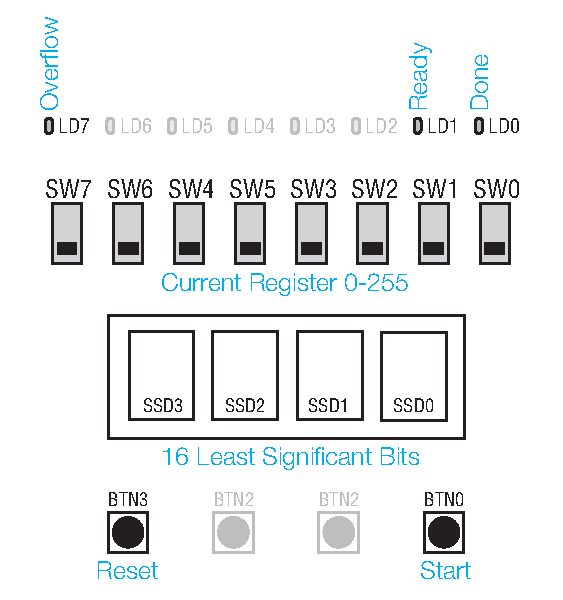
\includegraphics[width=75mm]{images/nexys2io.pdf}
  \caption{Input/output of the data explorer front-end for the FFT.}  
  \label{fig:io}
  \end{figure}
  
  \subsection{Data Explorer}
  In the data explorer mode, the switches act as binary inputs, allowing the user to address all 256 registers. The four SSD
  displays show the least significant bits of the selected register. In the event of overflow, \lstinline!LD7! will light up.  The user
  may explore the initial data, then press \lstinline!Btn0! to perform the Fast Fourier Transform of the data.
  
  In the final implementation, the butterfly unit (combinational logic) was separated from the index pointer logic. Block memory, 
  in this case two instances of dual-port RAM, were used in place of registers, which improved the speed of synthesis at the
  cost of clock cycles.  The final resource usage is summarized in table \ref{tab:usage}. The minimum period is 13.8 ns (72.14 MHz)
  and the critical path runs through the butterfly unit.
  
  \begin{table}[h]
  \begin{tabular}{l  r  r  r}
                                        & Used  & Avail. & Perc. \\
   Number of Slices:                    &  684  & 4656  &  14\%  \\
   Number of Slice Flip Flops:          &  198  & 9312  &   2\%  \\
   Number of 4 input LUTs:              & 1316  & 9312  &  14\%  \\
   Number of IOs:                       &   37  &       &      \\
   Number of bonded IOBs:               &   36  &  232  &  15\%  \\
   Number of BRAMs:                     &    2  &   20  &  10\%  \\
   Number of MULT18X18SIOs:             &   10  &   20  &  50\%  \\
   Number of GCLKs:                     &    2  &   24  &   8\%  \\
 \end{tabular}
 \caption{Resource usage.}
 \label{tab:usage}
 \end{table}
  
  
  
  \subsection{The Inverse Transform}
    After manipulating the signal in the frequency domain, we must transform back into the time domain for playback. 
    Rather than implementing a separate IFFT module, we can reuse the FFT module.  We simply switch the real and imaginary
    inputs and divide the final result, which will be located in the imaginary data, by 1024.

%
%
% Phase vocoder
%
%
\section{Phase Vocoder}
  The most basic way of shifting pitch is to simply speedup or slowdown the playback. For instance, we can shift the pitch
  by one octave if we playback twice as fast.  
  However, this is undesirable because the duration will now be twice as short.  
  The phase vocoder allows us to change the pitch of a signal without affecting speed.
  It makes use of the Short-Time Fourier Transform to analyze a segment of the input signal, scales the frequencies accordingly,
  and outputs the modified signal using the overlap-add method. The process is shown in figure \ref{fig:vocoder}.
  \begin{figure}[h]
  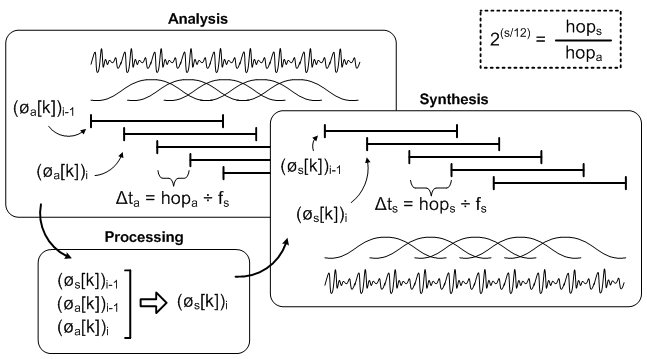
\includegraphics[width=75mm]{images/vocoder.png}
  \caption{Processes involved in a phase vocoder \cite{bib:guitarpitchshifter}.}  
  \label{fig:vocoder}
  \end{figure}
  
  However, this technique introduces audio artifacts at the edges of overlaps.  Therefore, we also multiply our input
  segment with a Hanning window, which is a cosine function that resembles a bell curve.  This helps smooth the output
  signal.
  
  \subsection{Proposed Hardware Implementation}
  Our design would take a 1024 bit chunk from the input audio register and transfer it to an intermediary register on which to perform
  various calculations. Each window chunk will be windowed, run through the FFT module, have the various phase and magnitude values
  calculated, run through the IFFT module, and then become windowed again with the phase and time changes in place. They can then either 
  be placed back in the original register, or a specific output register. 
  
%
%
% Conclusion
%
%
\section{Conclusion}
We have created an FFT module in Verilog and a simple phase vocoder using \textsc{Matlab}. There are many possible uses for such a device that can be achieved
with minor modifications. A basic guitar pitch shifting pedal can be made if the effect can be applied live. 
To increase the speed of the process, we can add more Butterfly units to reduce the amount of time needed in the FFT.  
If we add a pitch detector, we can create an auto-tuner. As of now, our design has a limitation of only scaling an octave, for the future
we would implement an algorithm to linearly interpolate values in order to scale at different factors. There are also various optimizations
that can be made if given more time. Although our design has a low power consumption and uses the clock time efficiently, it is slower 
to implement.

\bibliographystyle{IEEEbib}
\begin{thebibliography}{10}
\bibitem[1]{bib:guitarpitchshifter} \url{http://guitarpitchshifter.com/}
\bibitem[2]{bib:mathworldfft} \url{http://mathworld.wolfram.com/FastFourierTransform.html}
\bibitem[3]{bib:ctdft} 	Cooley, J. W. and J. W. Tukey, ``An Algorithm for the Machine Computation of the Complex Fourier Series," Mathematics of Computation, Vol. 19, April 1965, pp. 297-301.
\bibitem[4]{bib:butterfly} Takala, J. and K. Punkka, ``Butterfly Unit Supporting Radix-4 and Radix-2 FFT," \url{http://ticsp.cs.tut.fi/images/4/48/Cr1028-riga.pdf}
\bibitem[5]{bib:fftdit} \url{http://cnx.org/content/m12016/latest/}
\bibitem[6]{bib:ffttricks} \url{http://cnx.org/content/m12021/latest/}
\end{thebibliography}
\end{document}